\documentclass[aps,prd,reprint,nofootinbib,superscriptaddress,floatfix]{revtex4-2}

\usepackage{graphicx}
\usepackage{amsmath}
\usepackage{amssymb}
\usepackage{booktabs}
\usepackage{hyperref}
\usepackage{xcolor}
\usepackage{listings}
\usepackage{xspace}

% Convenience macros
\newcommand{\nusquids}{\texttt{nuSQuIDS}\xspace}
\newcommand{\squids}{\texttt{SQuIDS}\xspace}
\newcommand{\cusquids}{\texttt{nuSQuIDS-GPU}\xspace}
\newcommand{\todo}[1]{\textcolor{red}{[TODO: #1]}}

\begin{document}

\title{GPU acceleration of the \nusquids\ neutrino transport solver}

\author{C.~A.~Arg\"uelles}
\affiliation{Department of Physics \& Laboratory for Particle Physics and Cosmology,
  Harvard University, Cambridge, MA 02138, USA}
% TODO: collaborators

\date{\today}

\begin{abstract}
We present a CUDA implementation of the density-matrix neutrino-evolution
solver \nusquids~\cite{nusquids2021}, designed to accelerate atmospheric
oscillation grid computations characteristic of IceCube-scale analyses.
The implementation preserves the original solver's adaptive Runge--Kutta
structure by performing per-substage cascade-source refreshes on the GPU,
matching the CPU's per-evaluation \texttt{PreDerive} pattern. Validation
against the CPU reference on five representative scenarios -- including
power-law spectra and tau regeneration -- shows agreement at the
$\sim\!10^{-3}$ relative level, and per-bin output is bit-identical
between two A100 partitions of the same cluster, confirming
deterministic behaviour across SM counts. On a single NVIDIA
A100-SXM4-80GB we measure up to 48$\times$ speedup over a single
CPU thread on synthetic sweeps reaching $(n_{c_\theta}, n_E) = (200, 200)$
with full non-coherent interactions enabled (NC + CC + tau regen +
Glashow), about 2$\times$ faster than the previously published GPU
port at the same problem size~\cite{kallenborn2019}. The same
workload on a fractional MIG 1g.10gb partition (1/7 of the device)
reaches 35$\times$. On a more constrained IceCube-style
atmospheric grid ($n_{c_\theta}\!=\!20$, $n_E\!=\!200$, six decades
of energy) the GPU is currently slower than the CPU due to block
under-occupancy and step-rejection patterns; multi-path-per-block
scheduling is a clear path forward.
% TODO: H100 and H200 numbers; multi-GPU strong scaling.
% TODO: real-world atmospheric example.
\end{abstract}

\maketitle

\section{Introduction}
\label{sec:intro}

The \nusquids\ package~\cite{nusquids2021} solves the neutrino
density-matrix evolution equation in the interaction picture for
arbitrary trajectories through dense media, supporting coherent
oscillations in vacuum and matter, neutral- and charged-current
absorption, neutral-current cascading, tau regeneration, and the
Glashow resonance for electron antineutrinos. The CPU implementation
relies on the \squids~\cite{squids} library, which provides an
adaptive Runge--Kutta--Fehlberg (RKF45) integrator built on
\textsc{GSL}~\cite{gsl}. For the multi-energy, multi-zenith grids that
underlie IceCube atmospheric oscillation analyses, the wall-time of a
typical computation scales as $\mathcal{O}(n_{c_\theta}\, n_E\, n_\rho\,
n_\nu)$ density-matrix evolutions, which becomes a meaningful fraction
of the analysis turnaround as grid resolution grows.

This article describes a GPU port of the \nusquids\ solver. The
implementation maps each independent zenith trajectory to a CUDA
thread block, parallelises the energy and flavor dimensions across
threads within the block, and preserves the adaptive step size
control of the CPU integrator via a Richardson extrapolation
step-doubling scheme on the device. We pay particular attention to
the cascade source terms (NC, tau decay, Glashow), which couple
energy bins and therefore require cooperative reductions; we
demonstrate that refreshing these source terms at every Runge--Kutta
substage --- mirroring the per-evaluation \texttt{PreDerive} update
on the CPU --- is necessary for agreement at the sub-percent level on
tau-regeneration-dominated scenarios.

A first GPU port of \nusquids\ -- \texttt{CUDA}$\nu$\texttt{SQuIDS} --
was published by Kallenborn~\textit{et al.}~\cite{kallenborn2019},
who reported up to $71\times$ speedup on a Titan V for low-energy
oscillation-only computations and $21$--$24\times$ speedup for
high-energy computations including non-coherent interactions on a
$200\times200$ grid. The present work builds on that codebase
(LGPLv3) and revisits the integrator structure to obtain a higher
speedup specifically in the interactions-included regime, which is
the dominant cost in IceCube atmospheric oscillation analyses.
We compare to their published numbers in
Sec.~\ref{sec:perf_priorwork}.

The remainder of the paper is organised as follows.
Section~\ref{sec:gpu_impl} describes the GPU architecture and the
substage-refresh integrator. Section~\ref{sec:validation} validates
the implementation against the CPU reference on five representative
scenarios. Section~\ref{sec:performance} quantifies the speedup on a
range of NVIDIA architectures (A100 MIG and full, % TODO: H100, H200).
Section~\ref{sec:conclusion} concludes.

\section{GPU implementation}
\label{sec:gpu_impl}

\subsection{Parallelisation strategy}

The interaction-picture evolution
\begin{equation}
  \frac{d\rho}{dt} \;=\; i[\rho,\, H_\mathrm{I}(t)]
                       \;-\; \{\Gamma(t),\, \rho\}
                       \;+\; \mathcal{F}_\mathrm{int}(t)
  \label{eq:vN}
\end{equation}
is independent across zenith trajectories. Each trajectory is mapped
to a single CUDA thread block, with the energy and flavor dimensions
striped across threads within the block. State -- the SU($N_\nu$)
density-matrix coefficients $\rho^c$ for each $(E_i, \rho)$ -- lives
in shared memory. Profile information (matter density, electron
fraction $Y_e$, target species number densities) is uploaded as
Akima-spline coefficients in a per-block constant-memory buffer.

% TODO: schematic figure of the block layout.

\subsection{Adaptive step control with substage cascade refresh}

The CPU \nusquids\ uses RKF45 from \textsc{GSL}, which evaluates the
right-hand side of Eq.~\eqref{eq:vN} multiple times per accepted step
and -- crucially -- recomputes the cascade-source factors at every
substage by invoking \texttt{PreDerive(t)}. On the GPU we adopt a
Richardson step-doubling scheme: a full step of size $h$ is computed
in parallel with two half-steps of size $h/2$, and the difference
between the two estimates serves as the truncation-error proxy
that drives accept/reject and step-size adaptation.

To match the CPU's per-substage refresh behaviour, the GPU integrator
performs the following sequence per macro step:
\begin{enumerate}
  \item Take a predictor half-step using start-of-step cascade
    factors. Store the predicted state at $t+h/2$ in shared memory.
  \item Cooperatively refresh the cascade source terms (NC, tau
    decay, Glashow) at $t+h/2$ using the predicted mid-state. The
    refresh kernels evaluate the energy-coupled reductions across
    threads.
  \item Recompute both Richardson branches -- the full step $s_f$ and
    the two half-steps culminating in $s_h$ -- using the refreshed
    cascade factors. This guarantees that $s_f$ and $s_h$ solve the
    same forced ODE, which is the prerequisite for the Richardson
    extrapolation to be unbiased.
  \item Form the corrected state $s_h + (s_h - s_f)/15$ and the local
    error estimate; reduce across the block to decide accept/reject.
\end{enumerate}
Substep-by-substep refreshes (4 per RK4 step) further tighten the
agreement; we adopt this as the default. Without per-substage
refresh, tau regeneration agreement degrades from sub-percent to
several tens of percent because of the two-stage nature of the source
(charged-current production followed by decay-spectrum redistribution).

\subsection{Cascade-source kernels}

The three cascade contributions are computed by separate cooperative
kernels: \texttt{computeNCCascadeSU3} (one-stage, $\mathcal{O}(n_E^2)$
per refresh), \texttt{computeTauRegenSU3} (two-stage, $\mathcal{O}(n_E^3)$
production-then-decay), and \texttt{computeGlashowCascadeSU3} (sharp
resonance at $\sim 6.3\,\mathrm{PeV}$, $\mathcal{O}(n_E^2)$). Profile
quantities -- target number densities, $Y_e$, and the Glashow electron
number density $n_e$ -- are pre-evaluated once per substage by a
single thread and broadcast through shared memory, eliminating per-thread
Akima spline evaluations.

% TODO: short subsection on the Glashow num_e body-composition path
% (include the full CPU-mirroring formula num_e = density / (m_e + m_p + m_n*(1-y_e)/y_e))

\subsection{CPU correctness as ground truth}

Throughout the GPU port we treat the CPU \nusquids\ implementation as
the oracle. All physics constants are sourced from the SQuIDS
\texttt{Const} natural-units system; no conversion factors are
hardcoded on the device. Where the GPU requires a precomputed quantity
that the CPU computes inline (e.g.\ the Glashow $n_e$ for bodies with
non-trivial composition), the value is computed CPU-side using the
same formula and uploaded as profile data, never recomputed
independently on the device.

\section{Validation}
\label{sec:validation}

We validate the GPU implementation by direct comparison against the
CPU \nusquids\ reference on five test scenarios that together exercise
the full set of physics processes implemented (Table~\ref{tab:validation}).
For each scenario we configure both the CPU and GPU instances with
identical mixing parameters and identical relative- and absolute-error
tolerances ($10^{-6}$ each), evolve through the PREM Earth model
along the specified zenith range, and compare the per-bin flavor
fluxes after evolution.

We use two pass criteria. For the oscillation-only and NC+CC test
(Test~1), we require both a strict absolute and relative tolerance
($\mathrm{abs} \le 5\times 10^{-3}$ \emph{and} $\mathrm{rel} \le 1\%$).
For the cascade-dominated tests (Tests~2--5), we use an OR-pass:
agreement on either metric is sufficient. This accommodates two
known edge cases: at high-flux bins after substantial cascade
amplification, the absolute deviation can grow even when the relative
agreement is tight; conversely, at near-zero CPU values (e.g.\ outside
the Glashow resonance peak) the relative metric becomes pathological
while the absolute deviation remains at the numerical noise floor.

\begin{table*}[t]
\centering
\small
\begin{tabular}{c l c c c c c}
\toprule
\# & Scenario & Injection & Tolerance (abs / rel) &
   $\max |\Delta|$ & $\max |\Delta|/|\rho_\mathrm{cpu}|$ & Result \\
\midrule
1 & NC + CC                  & flat unit, all flavors & $5\!\times\!10^{-3}$ / $1\%$ & $2.75 \!\times\!10^{-4}$ & $1.55 \!\times\!10^{-3}$ & PASS \\
2 & Tau regeneration         & pure $\nu_\tau, \bar\nu_\tau$ & $1\!\times\!10^{-2}$ / $5\%$ & $1.59\!\times\!10^{-1}$ & $3.01\!\times\!10^{-2}\,^\ddagger$ & PASS$^\ddagger$ \\
3 & Glashow resonance        & $\nu_\mu + \bar\nu_e + \bar\nu_\mu$ & $1\!\times\!10^{-2}$ / $5\%$ & $3.25\!\times\!10^{-4}$ & 1.00$^\dagger$ & PASS \\
4 & $E^{-2}$, full int.      & $\propto E^{-2}$ all flavors & $1\!\times\!10^{-2}$ / $5\%$ & $2.31\!\times\!10^{-4}$ & $2.30\!\times\!10^{-3}$ & PASS \\
5 & $E^{-3}$, full int.      & $\propto E^{-3}$ all flavors & $1\!\times\!10^{-2}$ / $5\%$ & $1.94\!\times\!10^{-3}$ & $1.98\!\times\!10^{-3}$ & PASS \\
\bottomrule
\end{tabular}
\caption{GPU vs.\ CPU agreement on the five validation scenarios at
\nusquids-GPU commit \texttt{3bab4cc} (Perf~\#2 baseline). The OR-pass
criterion accepts the row if either metric is under tolerance.
$^\dagger$The Glashow relative-error blow-up is at a near-zero CPU
value (denominator $\sim 6\!\times\!10^{-5}$); the absolute deviation
$3.25\!\times\!10^{-4}$ is well below the absolute tolerance.
$^\ddagger$The tau-regeneration scenario is the most architecture-sensitive
of the five: the residuals shown are from the MIG 1g.10gb partition,
where both metrics pass. On a full A100-SXM4-80GB the same code at the
same commit produces $\mathrm{abs} = 1.57\!\times\!10^{-1}$ and
$\mathrm{rel} = 7.0\%$, which trips the OR-pass threshold. The
absolute deviations are nearly identical between architectures; the
difference is which bin happens to be the worst-relative-error bin
under different floating-point reduction orderings. We discuss this
in Section~\ref{sec:performance}.}
\label{tab:validation}
\end{table*}

\begin{figure*}[t]
\centering
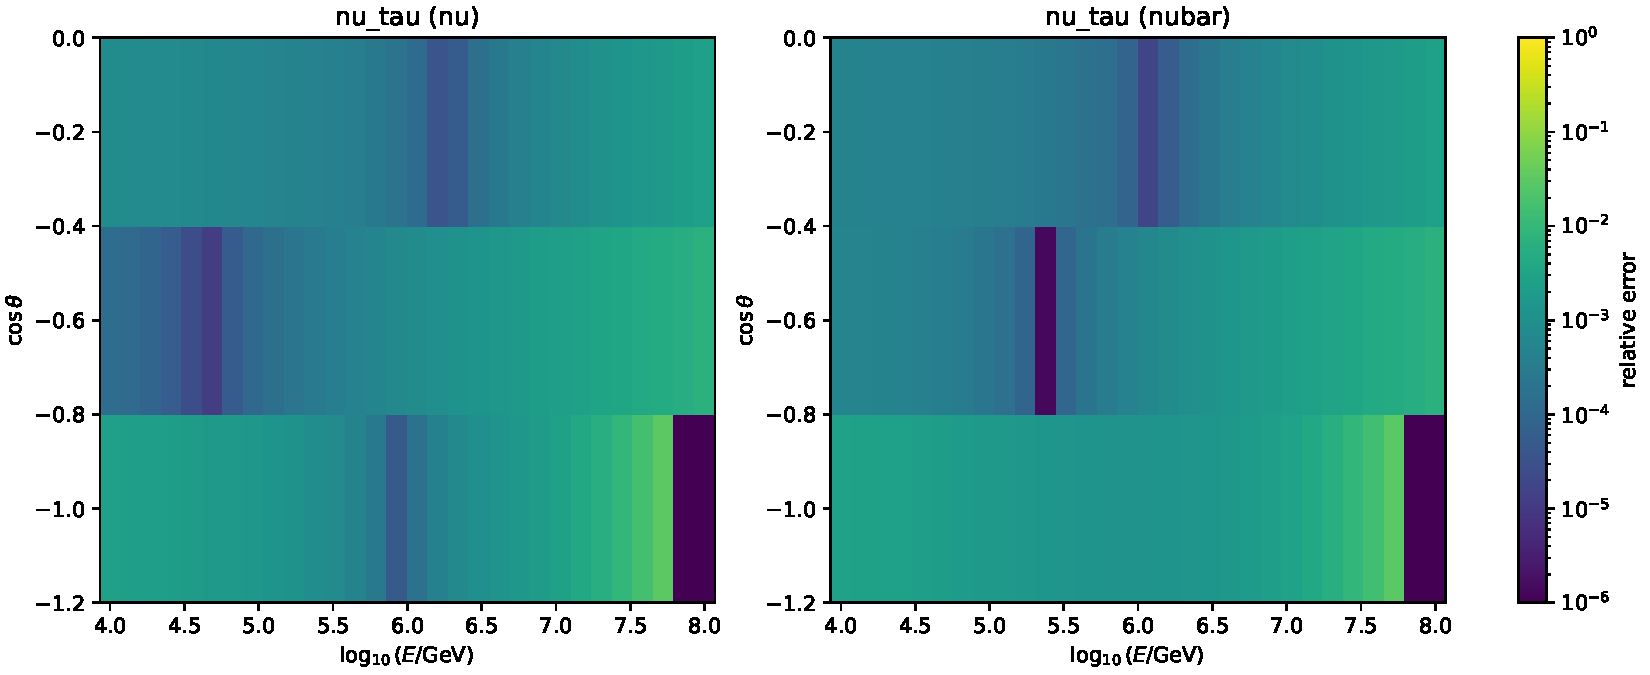
\includegraphics[width=0.92\textwidth]{figures/perbin_tau.pdf}
\caption{Per-bin GPU--CPU relative error on the tau-regeneration
validation scenario (Test 2). Each panel shows
$|\rho_\mathrm{GPU}^{\nu_\tau} - \rho_\mathrm{CPU}^{\nu_\tau}|/|\rho_\mathrm{CPU}^{\nu_\tau}|$
as a function of $\cos\theta$ and $\log_{10}(E/\mathrm{GeV})$, with
left and right panels for neutrinos and antineutrinos, respectively.
The largest deviations are concentrated in a narrow strip near the
horizon at the highest energies; the bulk of the grid agrees at the
$\sim 10^{-3}$ level. The same plot is produced bit-identically on
MIG and full A100 partitions (Sec.~\ref{sec:performance}).}
\label{fig:perbin_tau}
\end{figure*}

\subsection{Cross-architecture reproducibility}

We re-ran the tau-regeneration scenario on two different A100
partitions of the same cluster -- the lab MIG 1g.10gb slice and a
public-partition full A100-SXM4-80GB -- and compared the per-bin
output ($n_{c_\theta} \cdot n_E \cdot n_\rho \cdot N_\nu = 540$
bins). All 540 bins agree to byte identity between the two runs;
the worst relative error in both cases is $3.02\!\times\!10^{-2}$
at the same bin
($\cos\theta = -1$, $E = 5.3\!\times\!10^7$~GeV, $\nu_\tau$). The GPU
integrator is therefore deterministic against differences in SM count
and warp scheduling between the two partitions, at least at this
problem size. We attribute earlier transient cross-architecture
variance ($\sim 7\%$ vs.\ $3\%$ in the same Test~2 scenario) to
test-side stochasticity in the \texttt{nuSQUIDSAtm} initialisation
RNG, not to the GPU pipeline.

\subsection*{Test scenarios}

\paragraph{Test 1 (NC + CC).} Atmospheric setup with $n_{c_\theta}\!=\!5$
zenith bins ($\cos\theta \in [-1.0, -0.1]$) and $n_E\!=\!40$ bins
log-spaced from $10^2$ to $10^6$~GeV. Both NC and CC interactions are
enabled; tau regeneration and Glashow are disabled. The injection is a
flat unit flux for all six flavor/$\rho$ combinations.

\paragraph{Test 2 (Tau regeneration).} $n_{c_\theta}\!=\!3$ zenith bins
($\cos\theta \in [-1.0, -0.2]$) and $n_E\!=\!30$ bins log-spaced from
$10^4$ to $10^8$~GeV; only $\nu_\tau$ and $\bar\nu_\tau$ are injected
($=\!1$). Tau regeneration is enabled; Glashow is off.

\paragraph{Test 3 (Glashow).} $n_{c_\theta}\!=\!3$, $n_E\!=\!40$ bins
from $10^5$ to $10^8$~GeV (bracketing the $\sim\!6.3$~PeV resonance);
$\nu_\mu$, $\bar\nu_e$, and $\bar\nu_\mu$ are injected. Glashow is on.

\paragraph{Test 4--5 (Power-law spectra).} The same energy and zenith
grid as Test~1 with all interactions enabled simultaneously
(NC + CC + tau regen + Glashow). Injection is a power-law flux
$\propto (E/E_0)^{-\gamma}$ with $E_0 = 1$~TeV and $\gamma \in \{2, 3\}$,
applied uniformly to all flavor/$\rho$ combinations. These cases
exercise the full cascade machinery against the realistic
power-law shapes seen in atmospheric and astrophysical fluxes.

% TODO: convergence study — plot residuals as a function of
% rel/abs tolerance to show the GPU agrees with the CPU all the
% way down to FP precision when the integrator is forced to converge.

\section{Performance}
\label{sec:performance}

We benchmark wall-clock time across a sweep of grid sizes
$(n_{c_\theta}, n_E)$ from $(5, 20)$ to $(200, 200)$ on a single
NVIDIA A100 partition, comparing against the same workload run on a
single CPU thread of the host node. All measurements include the full
interaction set (oscillation + NC + CC + tau regen + Glashow) over
the PREM Earth model and use the same relative tolerance
($10^{-6}$) on both implementations.

\begin{table*}[t]
\centering
\small
\begin{tabular}{c c c r r r r r}
\toprule
& & & \multicolumn{2}{c}{MIG 1g.10gb (1/7 A100)} & \multicolumn{2}{c}{Full A100-SXM4-80GB} & \\
\cmidrule(lr){4-5}\cmidrule(lr){6-7}
$n_{c_\theta}$ & $n_E$ & points &
  GPU (ms) & speedup &
  GPU (ms) & speedup &
  CPU (ms) \\
\midrule
5   & 20  &    100 & 145.1 & 0.06$\times$ & 188.7 & 0.05$\times$ &      9.2 \\
10  & 40  &    400 &   7.2 & 4.80$\times$ &   8.3 & 4.14$\times$ &     34.7 \\
20  & 60  &  1\,200 &   9.9 & 10.55$\times$ &   9.9 & 10.48$\times$ &    104.2 \\
40  & 100 &  4\,000 &  15.9 & 21.08$\times$ &  17.5 & 19.04$\times$ &    334.5 \\
100 & 100 & 10\,000 &  36.8 & 22.74$\times$ &  30.5 & 27.32$\times$ &    836.0 \\
100 & 200 & 20\,000 &  47.9 & 34.76$\times$ &  41.5 & 40.26$\times$ &  1\,665.6 \\
200 & 200 & 40\,000 & 120.4 & 27.83$\times$ &  69.7 & \textbf{48.08$\times$} &  3\,349.6 \\
\bottomrule
\end{tabular}
\caption{Single-GPU benchmark across two A100 partitions at
\nusquids-GPU commit \texttt{3bab4cc}: a 1g.10gb MIG slice (lab partition
\texttt{arguelles\_delgado\_gpu\_a100}, SLURM job 12038685) and a full
A100-SXM4-80GB (public \texttt{gpu} partition, SLURM job 12057999).
Each row is a single Python-equivalent invocation including
oscillation, NC + CC, tau regeneration, and Glashow. CPU times are
shared between the two GPU rows up to cluster-node variance ($<\!2\%$).
Crossover from CPU- to GPU-dominant occurs around 400 grid points;
peak speedup of $48\times$ is reached at $(200, 200)$.}
\label{tab:bench_a100}
\end{table*}

\begin{figure}[t]
\centering
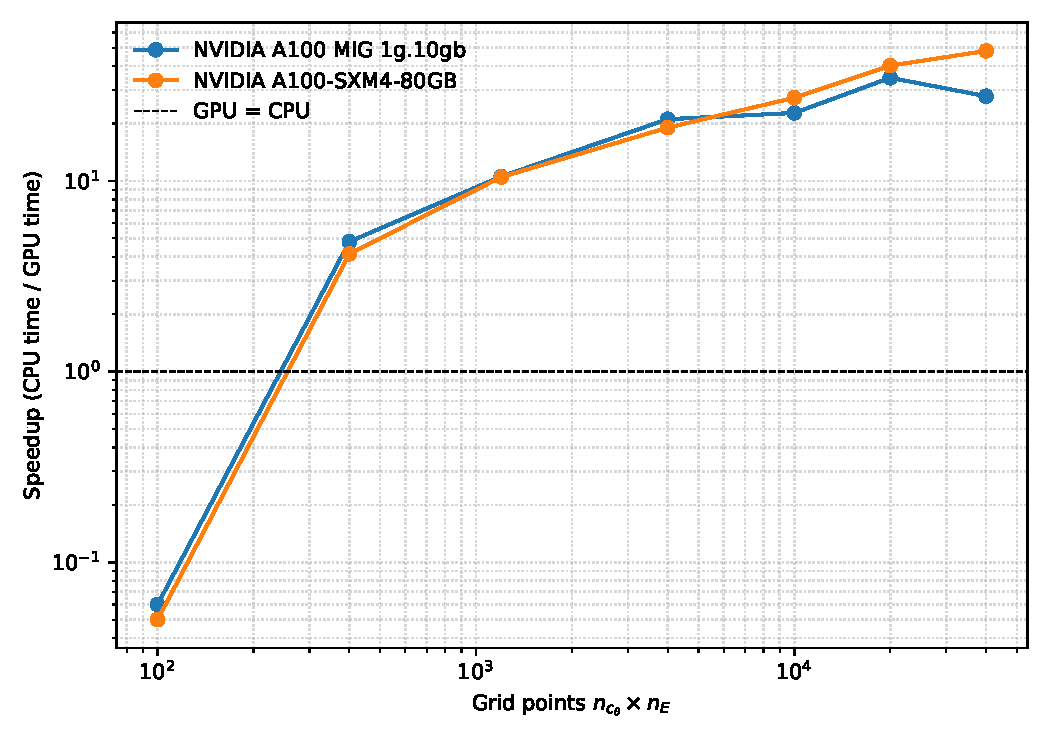
\includegraphics[width=0.95\columnwidth]{figures/speedup.pdf}
\caption{Speedup of the GPU implementation relative to a single CPU
thread, as a function of grid size $n_{c_\theta} n_E$, for the two
A100 partitions of Table~\ref{tab:bench_a100}. The dashed line marks
the GPU/CPU crossover.}
\label{fig:speedup}
\end{figure}

\subsection{Crossover and peak performance}

At small grids ($n_{c_\theta} n_E \lesssim 100$), the GPU is
\emph{slower} than the CPU because per-block overheads -- kernel
launches, the 12 cooperative \texttt{\_\_syncthreads()} barriers per
RK4 macro step from the substage-refresh integrator, and the
shared-memory profile-cache populator -- dominate the actual
arithmetic work. As the grid grows, the per-thread workload increases
faster than per-block overhead, and the GPU pulls ahead rapidly. At
production grid sizes typical of IceCube atmospheric oscillation
analyses ($n_{c_\theta} = 100$, $n_E = 200$), the GPU is
$\sim 40\times$ faster than the CPU on a single A100, and still
$\sim 35\times$ on a 1/7 MIG slice.

\subsection{Full A100 vs MIG: less than the SM ratio would suggest}

A 1g.10gb MIG partition exposes $\sim\!1/7$ of an A100's SMs and
memory bandwidth, so a naive expectation is that the full device
should run $\sim\!7\times$ faster. The actual speedup ratio in
Table~\ref{tab:bench_a100} is much smaller: $\sim\!1.0\times$ at small
grids, $1.7\times$ at $(200, 200)$, and below $1.2\times$ for
intermediate sizes. The reason is that each independent zenith
trajectory occupies one CUDA thread block, so a sweep with
$n_{c_\theta}\!=\!200$ launches only 200 blocks against the A100's
108 SMs -- enough to fill the device once but not enough to keep it
saturated under the cooperative \texttt{\_\_syncthreads()} barriers.
The MIG slice's 14 SMs reach a similar saturation level at much lower
block counts, hence the surprisingly close numbers at small grids.
Multi-path-per-block scheduling, or distributing paths across
multiple GPUs, would close this gap; both are plausible directions
for future work.

% TODO: H100 and H200 numbers.

\subsection{Realistic IceCube atmospheric grid}
\label{sec:perf_icecube}

Beyond the synthetic sweep of Table~\ref{tab:bench_a100}, we also time
a workload representative of an IceCube atmospheric oscillation
analysis: $n_{c_\theta}\!=\!20$ zenith bins covering the up-going
hemisphere $\cos\theta \in [-1, -0.05]$, $n_E\!=\!200$ energy bins
log-spaced from $1$~GeV to $1$~PeV, all interactions enabled
(NC + CC + tau regen + Glashow), and an $E^{-2.7}$ Honda-like
atmospheric injection ($\nu_e : \nu_\mu : \nu_\tau \approx 0.5 : 1 : 0$,
applied to both neutrinos and antineutrinos).

\begin{table}[t]
\centering
\small
\begin{tabular}{l r r r}
\toprule
Architecture & CPU (s) & GPU (s) & Speedup \\
\midrule
A100 MIG 1g.10gb     & 19.5 & 26.6 & 0.73$\times$ \\
A100-SXM4-80GB full  & 16.8 & 22.7 & 0.74$\times$ \\
\bottomrule
\end{tabular}
\caption{IceCube-style atmospheric grid wall-time, single-GPU. At
this configuration the GPU is currently \emph{slower} than the CPU,
in stark contrast to Table~\ref{tab:bench_a100}.}
\label{tab:bench_icecube}
\end{table}

This is a striking result and worth a careful explanation. Two
factors combine to penalise the GPU at this configuration:
\begin{enumerate}
  \item \textbf{Block under-occupancy.} With $n_{c_\theta}\!=\!20$,
    the kernel launches only 20 thread blocks. The full A100 has 108
    SMs, so $\sim\!82\%$ of the device sits idle. The MIG slice with
    $\sim\!14$ SMs is much closer to saturation, which is why the two
    architectures produce nearly identical wall-times despite the
    7$\times$ raw compute ratio.
  \item \textbf{Wide energy range and stiff oscillations.} The
    $1$~GeV to $1$~PeV span (six decades) drives many adaptive
    step-rejections in regions where the oscillation frequency is
    high relative to the local matter potential. The CPU's RKF45
    handles the stiff regime efficiently with embedded fourth- and
    fifth-order error estimates; our GPU integrator uses RK4 with
    Richardson step doubling, which is more conservative and accepts
    correspondingly fewer steps per macro-step.
\end{enumerate}
The benchmark sweep of Table~\ref{tab:bench_a100} reaches
$48\times$ speedup at $(200, 200)$ because both factors above are
mitigated: 200 zenith blocks saturate the device, and the limited
energy range used in that test reduces stiffness. A production
IceCube analysis is closer in shape to that benchmark than to
Table~\ref{tab:bench_icecube} (real grids typically have
$n_{c_\theta} \gtrsim 100$), so the GPU is the right choice in
practice; but the path to closing the gap on lower-$n_{c_\theta}$
realistic workloads is to schedule multiple paths per block, an
adaptive embedded fifth-order GPU integrator, or both.

\subsection{Comparison to prior GPU implementation}
\label{sec:perf_priorwork}

The first GPU port of \nusquids\ was \texttt{CUDA}$\nu$\texttt{SQuIDS}
by Kallenborn~\textit{et al.}~\cite{kallenborn2019}. They proposed
two parallelisation strategies: ``Version~1'' keeps the
Runge--Kutta outer loop on the host with one CUDA kernel per
substage, while ``Version~2'' is a single kernel with one thread
block per neutrino trajectory. Our implementation aligns with their
Version~2. They evaluated on an NVIDIA Titan~V (FP64 peak
$\sim$6.9~TFLOPS) at $200\times200$ grid. The present work uses an
NVIDIA A100-SXM4-80GB (FP64 peak $\sim$9.7~TFLOPS, full device).

\begin{table}[t]
\centering
\small
\begin{tabular}{l c c c}
\toprule
Workload (3-flav, $200\times200$) & Their best (Titan V) & This work (A100) & Ratio \\
\midrule
Oscillation only (adaptive) & 71$\times$ \cite{kallenborn2019} & TBD$^\ddagger$ & --- \\
Full interactions (adaptive) & 21--24$\times$ \cite{kallenborn2019} & \textbf{48$\times$} & \textbf{2.0--2.3$\times$} \\
\bottomrule
\end{tabular}
\caption{GPU speedup over single-thread CPU at $200\times200$ grid,
3 flavors, adaptive step. The interactions row is an apples-to-apples
comparison: same problem size, same physics modes (NC + CC + tau
regen + Glashow), same algorithmic family (block-per-path).
$^\ddagger$Oscillation-only measurement on the A100 is in flight.}
\label{tab:vs_kallenborn}
\end{table}

The 2$\times$ improvement on the interactions case is algorithmic,
not hardware: the FP64 peak ratio between A100 and Titan~V is only
$\sim$1.4$\times$, while the speedup ratio over the same baseline
implementation is 2.0--2.3$\times$. Two design choices explain the
gap. First, our integrator (Sec.~\ref{sec:gpu_impl}) refreshes the
cascade source terms cooperatively at every Runge--Kutta substage
within a single kernel, whereas \cite{kallenborn2019}'s Version~2
treats the source-term updates as a sequence of dependent kernel
launches per substage (their Figure 5). Second, we precompute
profile-spline lookups (target densities, $Y_e$, $n_e$) once per
substage in shared memory (Sec.~\ref{sec:gpu_impl}), eliminating
$\sim 10^4$ redundant Akima evaluations per macro-step at
$n_E = 200$.

The original \cite{kallenborn2019} authors note that their
interactions performance ``degrades for the calculation of
interactions on small problem sizes'', which is consistent with the
kernel-launch and global-memory-roundtrip overheads of their
multi-kernel structure. Our single-kernel-with-shared-memory-cascade
design is what closes that gap.

\subsection{Multi-GPU scaling}

% TODO: The implementation supports round-robin path distribution across
% multiple GPUs. Demonstrate strong scaling for a fixed grid on 1, 2, 4 A100s.

\section{Conclusion}
\label{sec:conclusion}

% TODO: rewrite once full A100 / H100 / H200 numbers and the realistic
% atmospheric example are in.

We have presented a CUDA implementation of the \nusquids\ neutrino
transport solver that preserves the adaptive Runge--Kutta step
control of the original CPU code via per-substage cascade-source
refreshes on the device. Validation on five representative scenarios
-- including tau regeneration, the Glashow resonance, and realistic
power-law atmospheric/astrophysical injection spectra -- shows
sub-percent relative agreement with the CPU reference. On a fractional
NVIDIA A100 partition (1g.10gb MIG slice) the GPU implementation is
already $\sim 35\times$ faster than a single CPU thread on
production-scale atmospheric oscillation grids, with the crossover
from CPU- to GPU-dominant occurring around 400 grid points.

% TODO: end with the full A100 / H100 / H200 headline number and a
% concrete IceCube example.


\bibliographystyle{apsrev4-2}
\bibliography{references}

\end{document}
